\section{List of model features/parameters and their biological foundation}

To write:
\begin{itemize}
    \item Table of parameters
    \item Lower apical surface area
    \item Shape of boundary condition
    \item Cell types extracted from data
    \item differential adhesion
    \item Nematic l1 for closing off
\end{itemize}
\section{Visual closeness}
While the Drosophila embryo has been studied for decades, it is only relatively recently conputer vision has gotten to a point where quantitative analyses of 5000 is feasible. Therefore the most vital thing to recuperate is the visual agreement between the morphology of simulation and data.

On the following page, the simulation and corresponding frames from [stas' paper] can be seen and compared:

\newpage

\begin{figure}[H]
    \centering
    \vspace*{-1cm}\hspace*{-1cm}\makebox[\textwidth]{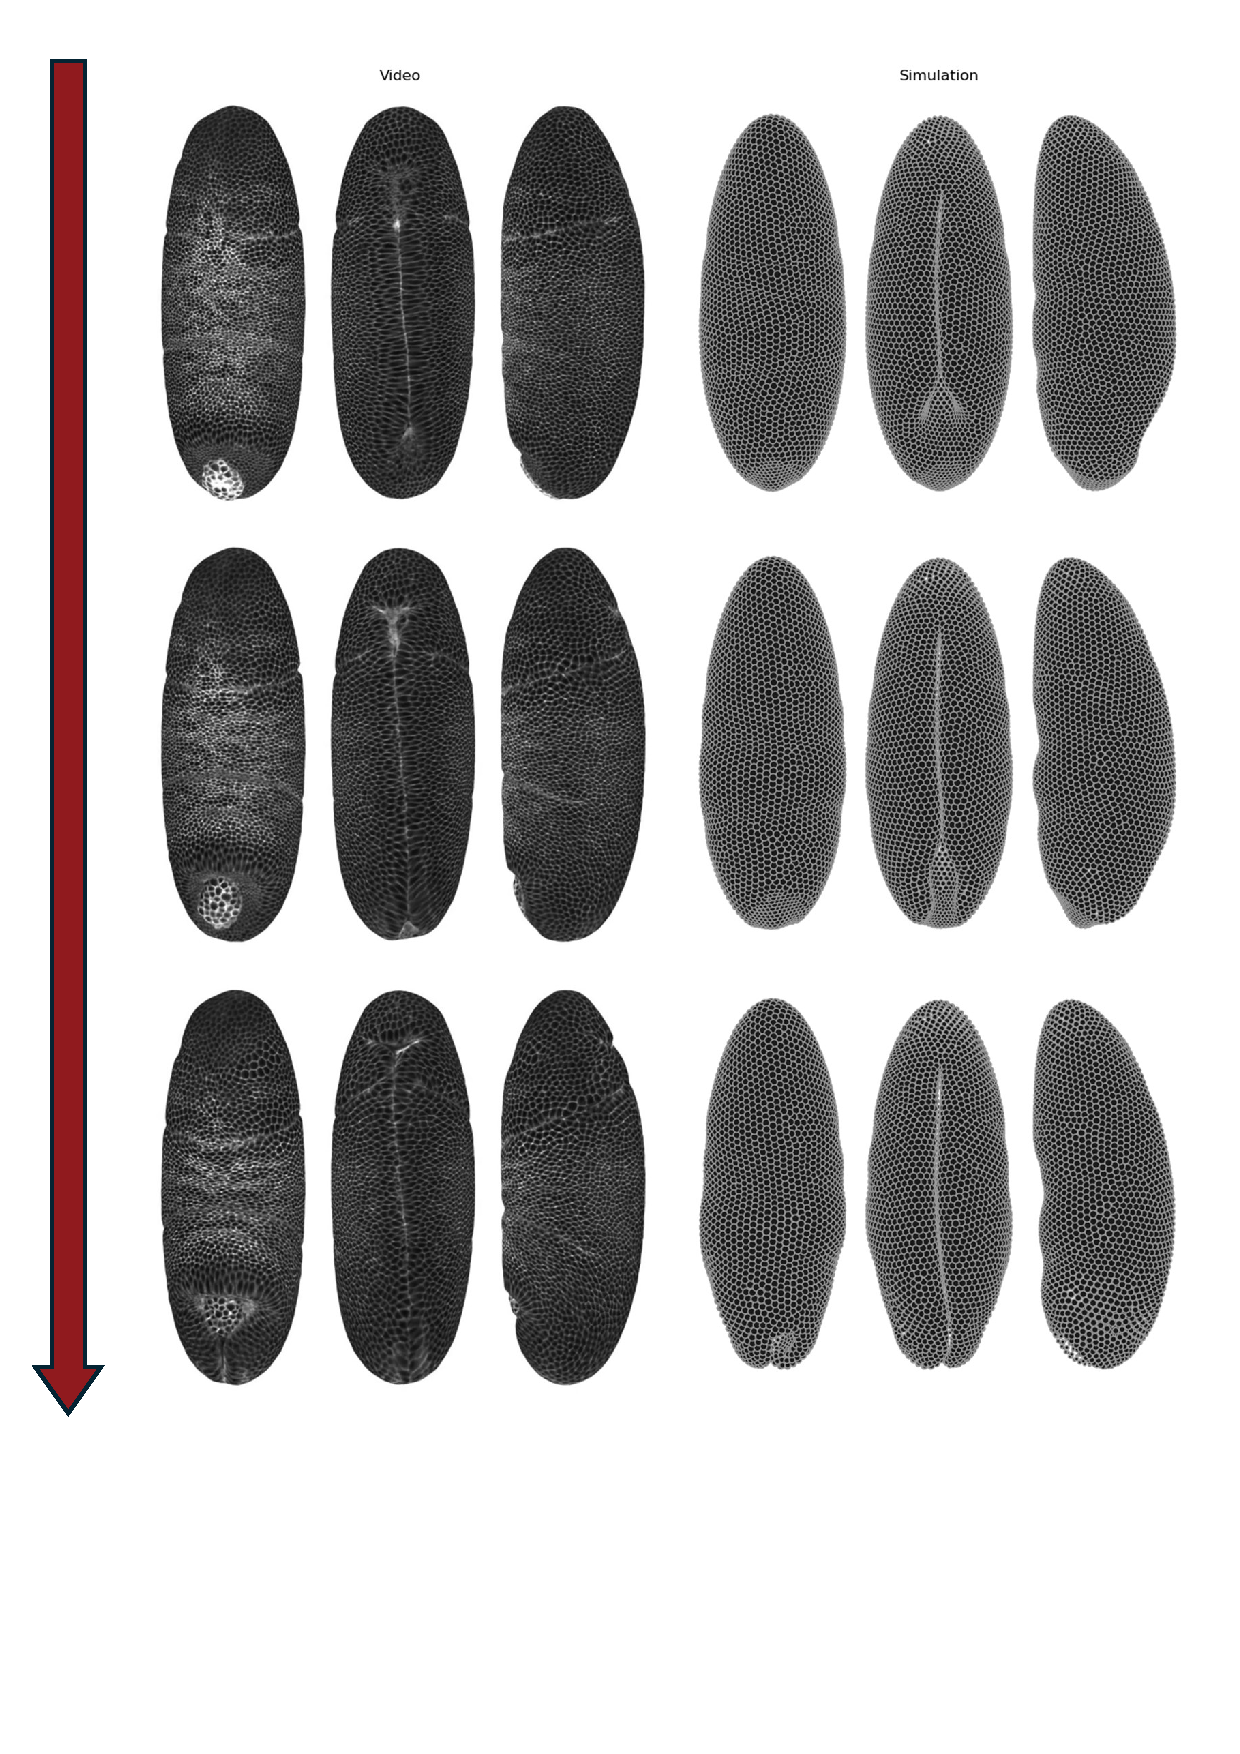
\includegraphics[width=0.85\paperwidth]{chapters/Results/figures/compare_to_vid_timeline.pdf}}
    \caption{Caption}
    \label{fig:enter-label}
\end{figure}
\newpage

\subsection{Ventral Furrow}
After mitosis stops, the the first visual change is on the belly, where a distinct cleft begins forming. \\

While all cells expressing \textit{twist} \& \textit{snail} lower their apical surface area, they do not constrict indiscriminately, instead starting with the \textit{inner} 8x60 cells.[citation needed] As the furrow closes off, creating closed-off tube with a recognizable light bulb-shape in the cross section, the tube extends dorsally.

In figure \ref{fig:VFComparison}, a comparison between a cross section of our simulation and in vivo imaging can be seen.

\begin{figure}[H]
    \centering
    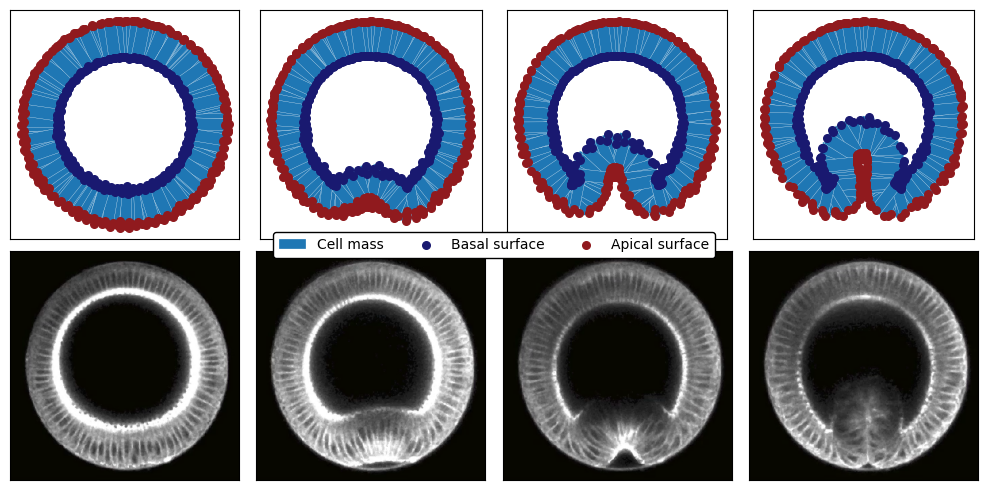
\includegraphics[width=1\linewidth]{chapters/Results/figures/VF_comparison.png}
    \caption{A comparison of simulation and frames from live development. \\\textbf{Upper row}: Simulation. \textbf{Lower row}: Multi-photon microscopy. \\For ease of visualisation, each cell in the simulation is displayed as a rectangle along its AB-axis. Each frame is taken at equally spaced time intervals. Cross section video borrowed from \cite{conte2012biomechanical}}
    \label{fig:VFComparison}
\end{figure}


Maybe quantify here?
I am guessing we can do a cell-center fit?
Out of scope? Yes. Would be cool? Also yes.
\subsection{Germ band}
The Germ Band is defined as the YYY. The general consensus is, that the Germ Band is the main driver of dorsal motion, although it remains disputed.

If Figure \ref{fig:germbandCompare} a diagram of the motion of the Germ Band can be compared with the shape of the Germ Band in the first and last frame of our simulation. 

\begin{figure}[H]
    \centering
    \begin{subfigure}[b]{0.34\textwidth}
        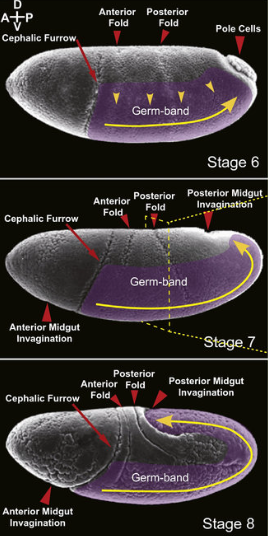
\includegraphics[width=\textwidth]{chapters/Results/figures/compareGB.png}
    \caption{Figure from \cite{kong2017forces} }
    \end{subfigure}
     \hfill
    \begin{subfigure}[b]{0.61\textwidth}
    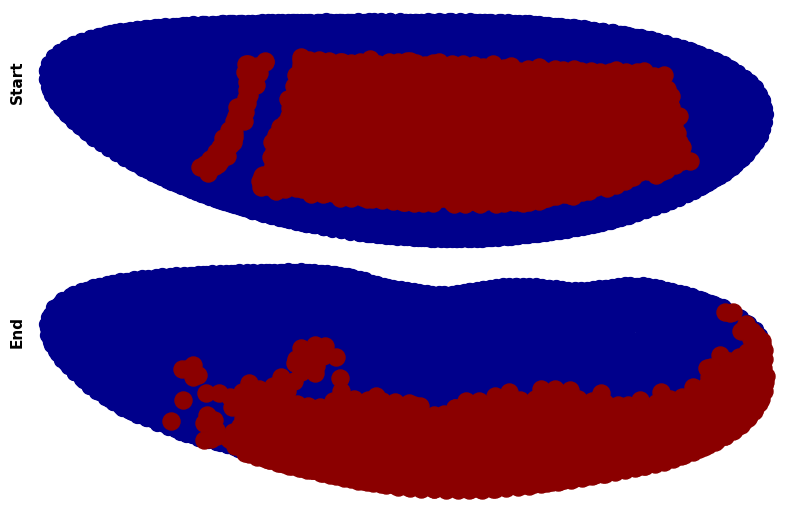
\includegraphics[width=\textwidth]{chapters/Results/figures/gb_firstframe_lastframe.png}
    \caption{Simulation}
    \end{subfigure}
    \caption{Colored in germ band for visual inspection.}
    \label{fig:germbandCompare}
\end{figure}

For an representation of the motions of the individual cells, see Figure \ref{fig:GBMovements} in the Appendix.
In general we see a great agreement between the morphological timeline of the germband between simulation and data.


\subsection{General morphology}
As way of visually seeing the changes in both local and global structure, drawing in straight lines before start of gastrulation and seeing how they translate and skew over time. An example of this (in both data and simulation can be seen in Figure \ref{fig:band-movements-stas}) 

\begin{figure}[H]
    \centering
    \makebox[\textwidth][c]{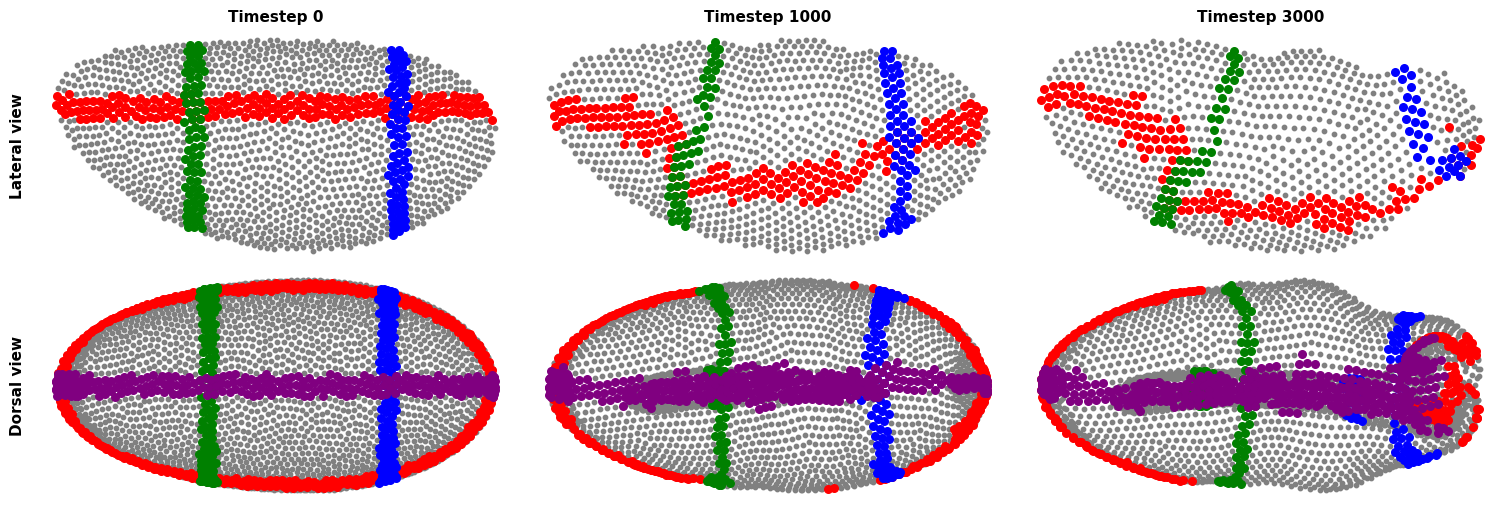
\includegraphics[width=1.1\linewidth]{chapters/Results/figures/band_movements.png}}
    % \caption{My simulation. Compare to figure \ref{fig:band-movements-stas}}
    % \label{fig:band-movements}
\end{figure}
\begin{figure}[H]
    \centering
    \makebox[\textwidth][c]{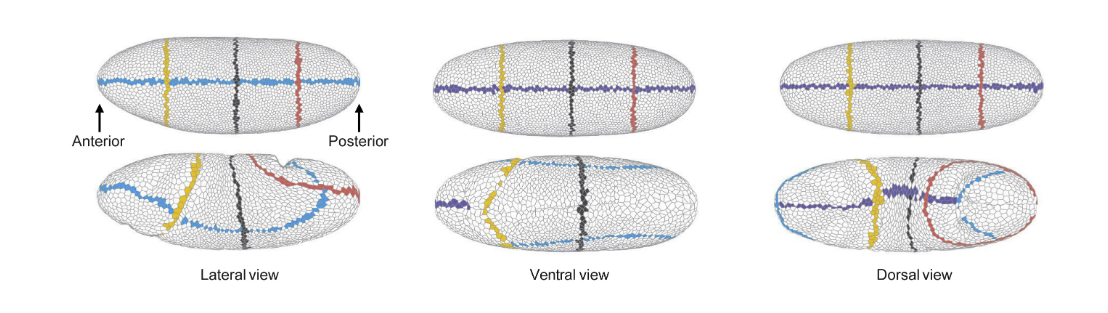
\includegraphics[width=1.\linewidth]{chapters/Results/figures/compareStasGBShape.png}}
    \caption{Position of specific bands over time.\\ \textbf{Top row:} Simulation | \textbf{Bottom row:}  Segmented images (from \cite{stern2022deconstructing}). \\\todo{make colors match.}}
    \label{fig:band-movements-stas}
\end{figure}

As is evident, the general agreement is pretty good :)


\subsection{Auxiliary furrows}

In the absence of controlled folding of the dorsal tissue, the pressure from the extending germband, can lead to other folds(?) \url{https://brunovellutini.com/posts/cephalic-furrow-thread/}

This is key to both understanding why the invaginated posterior end does not travel further anteriorly.

Also the large scale morhpology change some runs had.
\subsection{Daniel}
\section{Quantitative closeness}
\subsection{Movements}
While comparing the large scale morphogenesis visually is interesting, for better quantification of the model performance, the following measure was devised:

For ever n'th time-step, look at the recent motion of each cell. Compare each of these to the average motion vector of the 10 spatially closest cells in data. The resulting angle difference between 0 and $\pi$ is scaled to be between 0 and 1, with 1 being perfect agreement.

\begin{figure}[H]
    \centering
    \makebox[\textwidth][c]{
    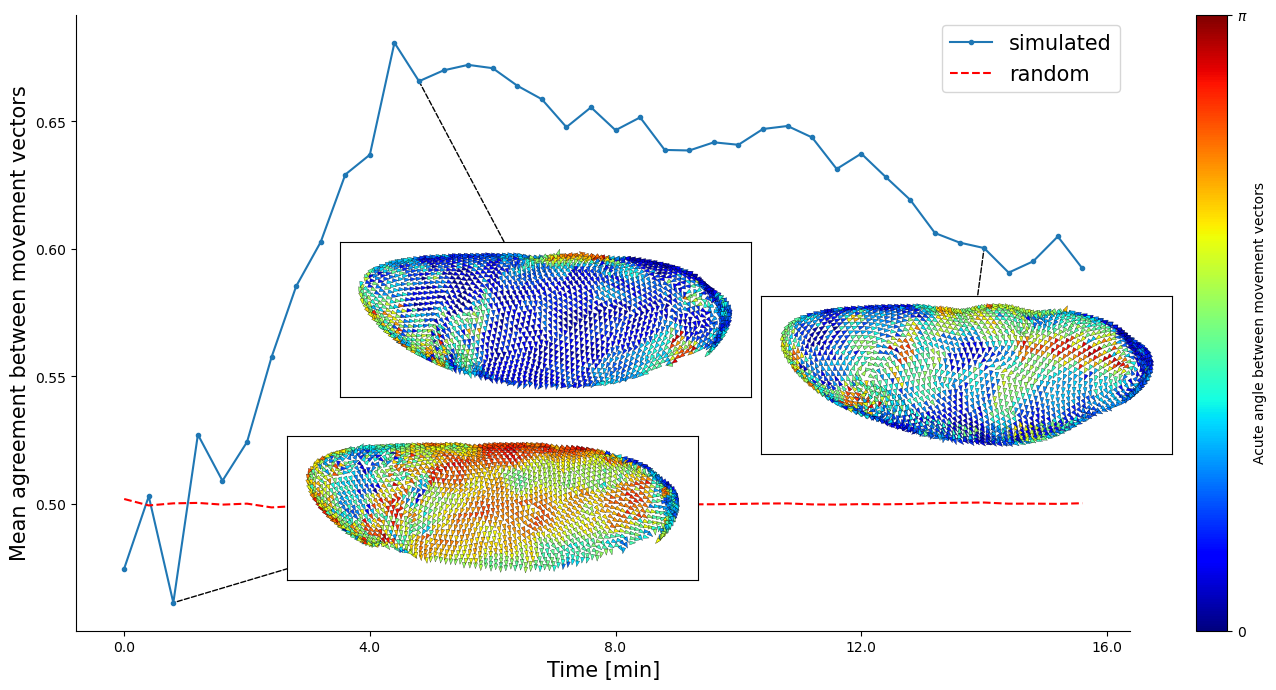
\includegraphics[width=1.3\linewidth]{chapters/Results/figures/movement_vectors_normal.png}
    }
    \caption{The motion-vector agreement across the full embryo as a function of time}
    \label{fig:motionAgreement}
\end{figure}

In general, we see a consistent, well-above average overlap. 


Important to note:
1) The data consist of machine-tracked cell positions. This means any radial motion is neglected.
2) Convergent extension is by its very nature based on the global motion being more important than the individual (see figure \ref{}) 

These two 



\subsection{Timing}
Cells have been shown to have remarkably precise internal clocks\footnote{cool footnote with a remarkable number\cite{cellinternal}} and chemical gradients in the embryo changing across timescales from seconds to hours\cite{shvartsman2008dynamics}. There is also the "biological clock"\cite{johanolsen2} that proteins themselves have dynamic structure that can change over time.\cite{johanolsen1}. But there is no evidence for any specific timing in stages 5-7 [citation needed]. The fact that our model seem have recapitulated much of the dynamics completely without any explicit time-dependent parameters seems to corroborate the fact that Boundary Conditions, Initial Conditions and an inter-atomic rule-set is sufficient for some of the complex morphology/anatomy to arise. 


\subsection{Strain}
As the tissue warps and skews the cells are both subject to- and drivers of- stress and strain on the cell walls. This is one of the most widely studied parts of structural changes in morphogenesis.

While our simulation neither includes cell walls nor explicit strain calculation, computer-vision method has been developed which we can utilize. The Green-Lagrangre algorithm, as utilized in \cite{butler2009cell} for example, looks at local deformations in the tissue. In figure \ref{fig:strain} the results of an implementation can be seen.

\begin{figure}[H]
    \centering
    \begin{subfigure}{0.45\linewidth}
        \centering
        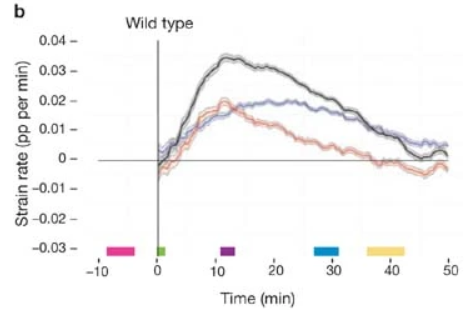
\includegraphics[width = \linewidth]{chapters/Results/figures/strain_rate_extrinsic.png}
    \end{subfigure}
        \begin{subfigure}{0.45\linewidth}
        \centering
        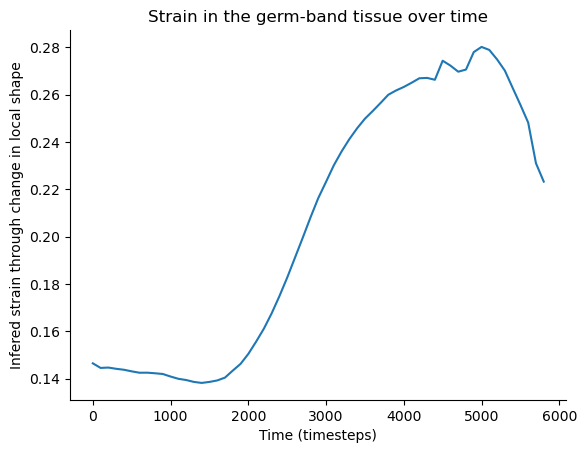
\includegraphics[width = \linewidth]{chapters/Results/figures/strain_smoothedpng.png}
    \end{subfigure}
    \caption{Comparison between Figure 1 from \cite{butler2009cell}. And an implementation of their strain-inference algorithm. Delayed onset, but quick rise followed by a fall-off at time of PMG invagination\\\todo{Explain the leftmost plot or find another that shows the same with only one line}}
    \label{fig:strain}
\end{figure}

"A strain rate is the ratio of the change in length to the original length, divided by the time interval, with units of proportion (pp) per minute. The lines show the mean strain rates for all five embryos, and the ribbon width represents the average standard error within a data set. The timing of developmental landmarks is shown for the five embryos recorded"

It can be seen in the first 12-15-minutes which we are, we see a rising strain, ending at the point of internalization of the germ cells. 

\subsection{Rosettes}
\begin{figure}[H]
    \centering
    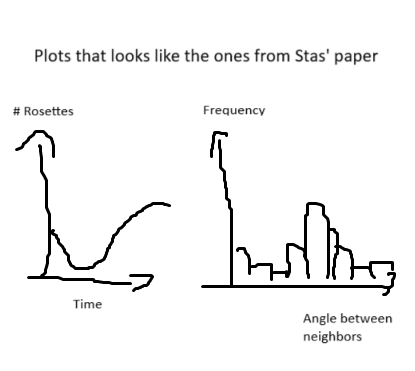
\includegraphics[width=0.8\linewidth]{chapters/Results/figures/rosettes_placeholder.png}
    \caption{Caption}
    \label{fig:enter-label}
\end{figure}

\begin{figure}[H]
    \centering
    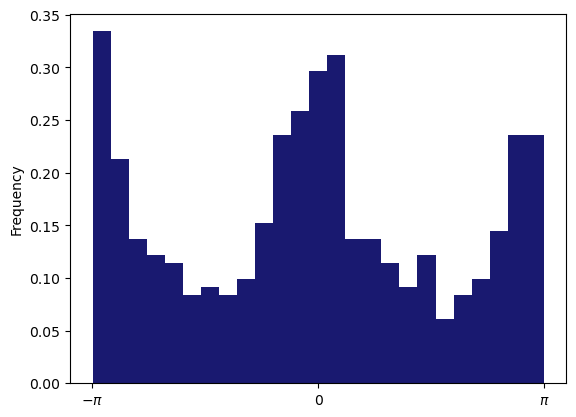
\includegraphics[width=0.6\linewidth]{chapters/Results/figures/rosettes_angle_dist.png}
    \caption{Caption}
    \label{fig:enter-label}
\end{figure}
\subsection{Daniel-data?}
\begin{figure}[H]
    \centering
    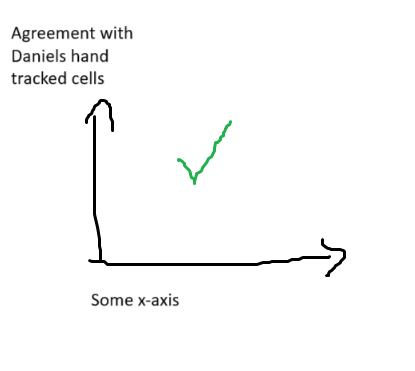
\includegraphics[width=0.8\linewidth]{chapters/Results/figures/daniel_placeholder.png}
    \caption{Caption}
    \label{fig:enter-label}
\end{figure}
\newpage
\section{In Silico Mutant "predictions" - compared to phenotypes and reference model}
Having a [pipeline] from (simplified) morphogen to (approximate) morphogenesis, opens the door for some intriguing explorations into our model and its relation to nature.

A large branch of developmental biology experiments consist of discovering or creating genotypes, and cataloging the resulting organisms. The genetic markup of animals that are deficient in some YYY. 
Our model allows for the creation of genetically-variant, by changing the response to one or more of the simulated morphogens.\\


\subsection{No PMG}
In [cite Stas] and [cite Stas again], they show that the chemical signals produced by the protein \textit{Hkb} are initiates the formation of the midgut by wavelike patterns of isotropic apical constriction around the posterior tip. In \textit{Hkb}-deficient mutants the lack of posterior invagination has a clear response. The build up pressure from the extending germ-band causes the . This has given the \textit{Hkb}-mutant the nickname "corkscrew mutant"\footnote{Timmy Glenn}.\\

In Figure \ref{fig:corkscrew-comparison}, a video of the corkscrew mutant can be compared to our simulation after removing the cells ability to react to \textit{Hkb}.

 
\begin{figure}[H]
    \centering
    \makebox[\textwidth][c]{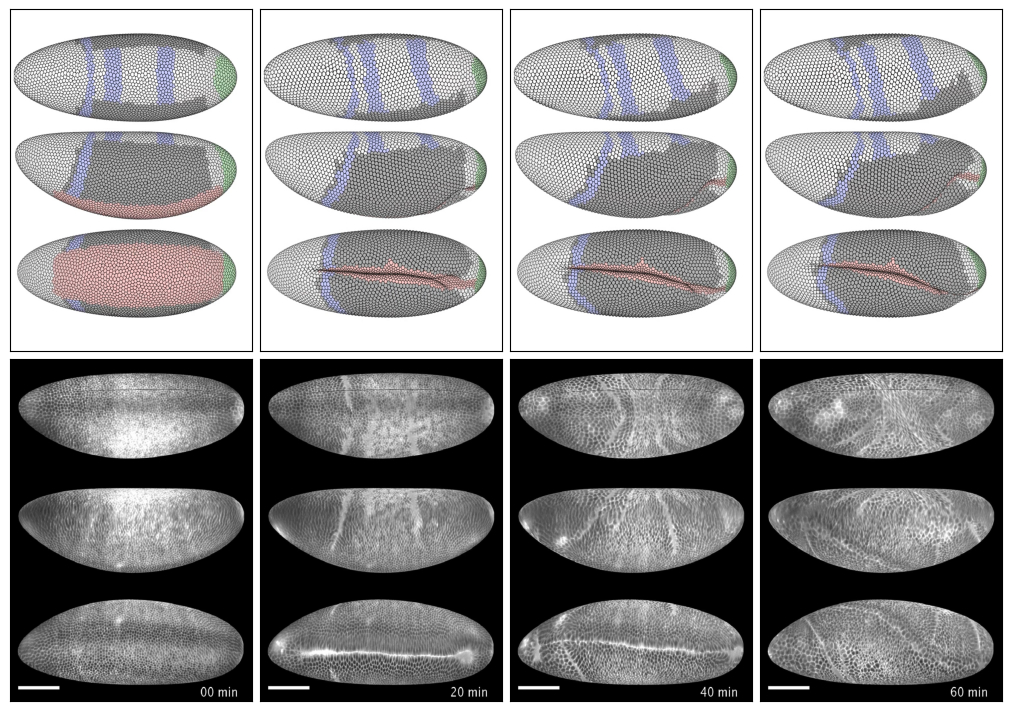
\includegraphics[width=1.2\linewidth]{chapters/Results/figures/corkscrew_comparison.png}}
    \caption{Comparing the \textit{Corkscrew} phenotype with my simulation. Video taken from \cite{smits2023maintaining}.}
    \label{fig:corkscrew-comparison}
\end{figure}
% Twist and shout

Comparing the reaction of these In Silico Mutants to real life phenotypes gives us a hint of capturing more than we we put in. TODO: make sound good. 

\subsection{No Ventral Furrow}
When knocking out the \textit{Twist} and \textit{Snail} genes, which, as you might remember, are primary organizers of apical constriction, the ventral furrow fails to form. 
% \url{https://genesdev.cshlp.org/content/5/9/1568.full.pdf}
% We are seeing the right thing
We are seeing the right thing.


\subsection{No Cephalic Furrow?}
not important
\subsection{No active intercolation / Germ band}
\label{sec:mutantNoGB}
We know that \textit{Runt} and \textit{Even skipped} are upstream . The litterature is conflicted, but the general theory is, that the patterning allows for a coherent orientation of the planar cell polarity. 

PCP-orientation was set at the intial step of the simulation as pointing in the distinct direction defined by the interspersed \textit{Runt} and \textit{Even skipped} patterning.
The results are interesting, albeit very uneventful, as
In the litterature  \cite{butler2009cell} more the morphogenesis is driven by more than Convergent Extension, and unstriped mutants are still viable, unlike our case where nothing happens.

Seems to be a clear indicator for active cell shape change being a vital part of... 

TODO: Discuss level of abstraction in the model 

\section{Combining and comparing to each other}
Given that we have a world-first [citation needed] full embryo model. Even with its flaws, in silico experiments by seeing how the different dynamical parts of the embryo interacts can be very interesting. \todo{omformulér}

We will be doing it, both by comparing the different 'phenotypes' to our baseline model, i.e. seeing how important the cell types are for a gastrulation that is comparable to the current best.

We introduce the metric \textit{Pole Cell Migration} as a virtual metric for the success of the gastrulation. The Pole Cell Migration is defined as the percentual angle change of the posterior tip in the lateral plane \todo{make figure? or just explain better}. As we have seen, the slow start followed by a sudden push seems to be a defining characteristic for the gastrulation. In Figure \ref{fig:PCM-mutants} a comparison of multiple runs of the "simple" mutants. \note{maybe no need to introduce PCM as a shorthand}

\begin{figure}[H]
    \centering
    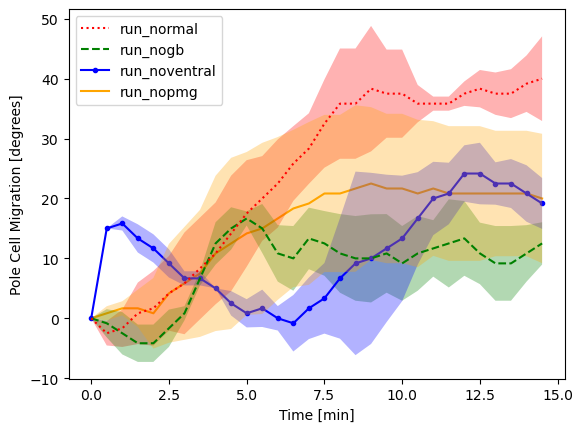
\includegraphics[width=1.\linewidth]{chapters/Results/figures/compare_PCM.png}
    \caption{\todo{Explain, fix x-axis}}
    \label{fig:PCM-mutants}
\end{figure}

Videos of the individual runs can be found in Section \ref{App:videos} in the Appendix, but a lot of the dynamics of the system can be gathered from the motion of the posterior tip. We can se that:
\textbf{Normal:} \\
\textbf{No Germband:} Without the pressure form the actively expanding germband, the motion purely from the invaginations. As the ventral cells also had $\lambda_3>0$ the there is still a tendency to move the tip dorsally, but there is not enough force for the posterior tip to move away from the [krængende]\todo{Translate} end of the egg allowing for the iconic [indfold]. \\
\textbf{No Ventral Furrow:} When we remove the VF-cells from the equation, the germ-band extends is not moved ventrally. This means they exert their pressure uniformly from the port and starboard sides not translating in the plane we are looking at.\\
\textbf{No PMG:} Here we see a possible breakdown of this metric, as, just like the in vivo experiments has show, the posterior tip moves slightly . None of the corkscrew-twising is captured. Not knowing how bad  50\% too little pole cell migration is, it does not capture just how unviable an embryo with this mutation is.   \\
\todo{This is very jovial, rewrite but keep same points.}\\


Now for a more granular approach, we boil the PCM down to a single number quantifying the total dorsal motion. In the matrix in Figure \ref{fig:PCM-matrix} we have calculated\footnote{emitting about 7kg of CO2 \url{https://mlco2.github.io/impact} } the combined effects of missing any two can be seen. 

\begin{figure}[H]
    \centering
    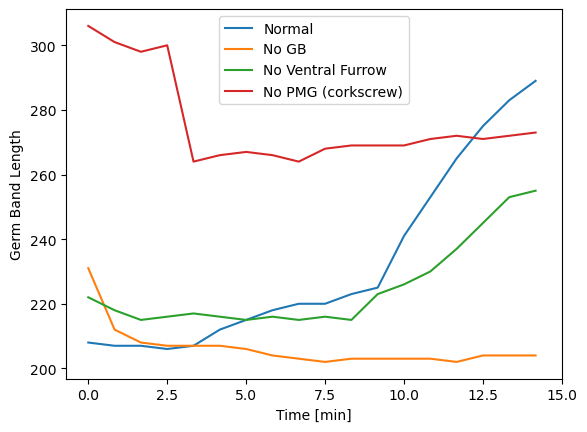
\includegraphics[width=1.\linewidth]{chapters/Results/figures/GB_len_mutants.png}
    \caption{Caption}
    \label{fig:PCM-matrix}
\end{figure}

\todo{Find something interesting to discuss}

\section{Combining and comparing to data}
While comparing internally is interesting and can say a lot about the dynamics, we wanted a short detour where we recreate Figure \ref{fig:motionAgreement}, seeing how each mutation changes the motion-vectors.

\begin{figure}[H]
    \centering
    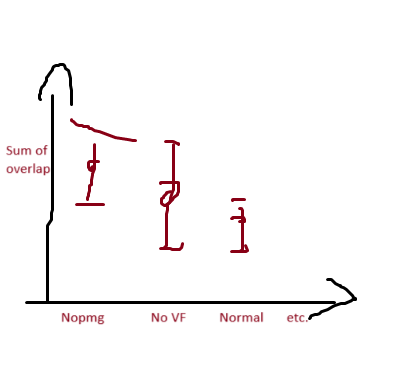
\includegraphics[width=1.3\linewidth]{chapters/Theory/figures/MutantDifference_Placeholder.png}
    \caption{This is the main plot of the thesis. Y-axis is sum of y-axis of over all times in Figure \ref{fig:motionAgreement}}
    \label{fig:enter-label}
\end{figure}
It is comforting to see,
\todo{Find something interesting to discuss}

\section{Parameter Sensitivity Analysis}
No good YY of a simple model is complete without a Paramater Sensitivity Analysis.





% \url{https://softmath.seas.harvard.edu/wp-content/uploads/2019/10/2009-07.pdf}
% clear that model is missing cell shape change!
% \section{Additive/subtractive working together matrix}
% \subsubsection{}